% =====================================================================
%  Clock / Timing diagrams for the documentation  (clean version)
%  Two cropped pages:
%    PAGE 1 = BEFORE : two independent FCLK roots -> HOLD VIOLATION
%    PAGE 2 = AFTER  : single MMCM root           -> HOLD MET
%  Compile on Overleaf / Prism (standalone -> each tikzpicture = 1 page).
% =====================================================================
\documentclass[tikz,border=14pt]{standalone}
\usepackage{amsmath}
\usepackage{amssymb}        % \checkmark
\usetikzlibrary{positioning,calc,arrows.meta,backgrounds}

% ---------- colour palette ----------
\definecolor{cmpute}{HTML}{1F6FB2}   % blue
\definecolor{memr}{HTML}{C0392B}     % red   = hold violation
\definecolor{dark}{HTML}{222B33}
\definecolor{grn}{HTML}{2E8B57}      % green = hold met
\definecolor{lblue}{HTML}{D6E6F4}
\definecolor{lred}{HTML}{F6DEDB}
\definecolor{lgrn}{HTML}{DDF0E5}
\definecolor{lgrey}{HTML}{ECF0F3}
\definecolor{mgrey}{HTML}{6B737B}

% ---------- shared styles ----------
\tikzset{
  ttl/.style    ={font=\sffamily\bfseries\large, text=dark},
  sub/.style    ={font=\sffamily\bfseries\small, text=mgrey},
  ff/.style     ={draw=dark, line width=1pt, rounded corners=2pt, fill=lblue,
                  text=dark, align=center, minimum width=1.7cm, minimum height=1.0cm},
  cmb/.style    ={draw=dark, line width=1pt, rounded corners=9pt, fill=lgrey,
                  text=dark, align=center, minimum width=1.8cm, minimum height=1.0cm},
  src/.style    ={draw=dark, line width=1pt, rounded corners=2pt, fill=white,
                  text=dark, align=center, minimum width=2.0cm, minimum height=0.95cm},
  mmcm/.style   ={draw=grn, line width=1.4pt, rounded corners=2pt, fill=lgrn,
                  text=dark, align=center, minimum width=2.1cm, minimum height=1.0cm},
  data/.style   ={-{Stealth[length=3mm]}, line width=1.1pt, draw=dark},
  clk/.style    ={-{Stealth[length=2.6mm]}, line width=1pt, draw=cmpute},
  clkg/.style   ={-{Stealth[length=2.6mm]}, line width=1pt, draw=grn},
  divider/.style={draw=mgrey!55, line width=0.6pt, dashed},
  badnote/.style={draw=memr, line width=1pt, rounded corners=3pt, fill=lred,
                  text=memr, align=center, font=\sffamily\small, text width=3.0cm},
  goodnote/.style={draw=grn, line width=1pt, rounded corners=3pt, fill=lgrn,
                  text=dark, align=center, font=\sffamily\small, text width=3.0cm},
  badchip/.style ={draw=memr, line width=1.2pt, rounded corners=4pt, fill=memr,
                  text=white, align=center, font=\sffamily\bfseries, inner sep=7pt},
  goodchip/.style={draw=grn, line width=1.2pt, rounded corners=4pt, fill=grn,
                  text=white, align=center, font=\sffamily\bfseries, inner sep=7pt},
  lab/.style    ={font=\sffamily\small, text=dark, align=center},
  labr/.style   ={font=\sffamily\small, text=memr, align=center},
  labg/.style   ={font=\sffamily\small, text=grn!45!black, align=center},
}

\begin{document}

% =====================================================================
% PAGE 1  --  BEFORE : two independent roots  ->  HOLD VIOLATION
% =====================================================================
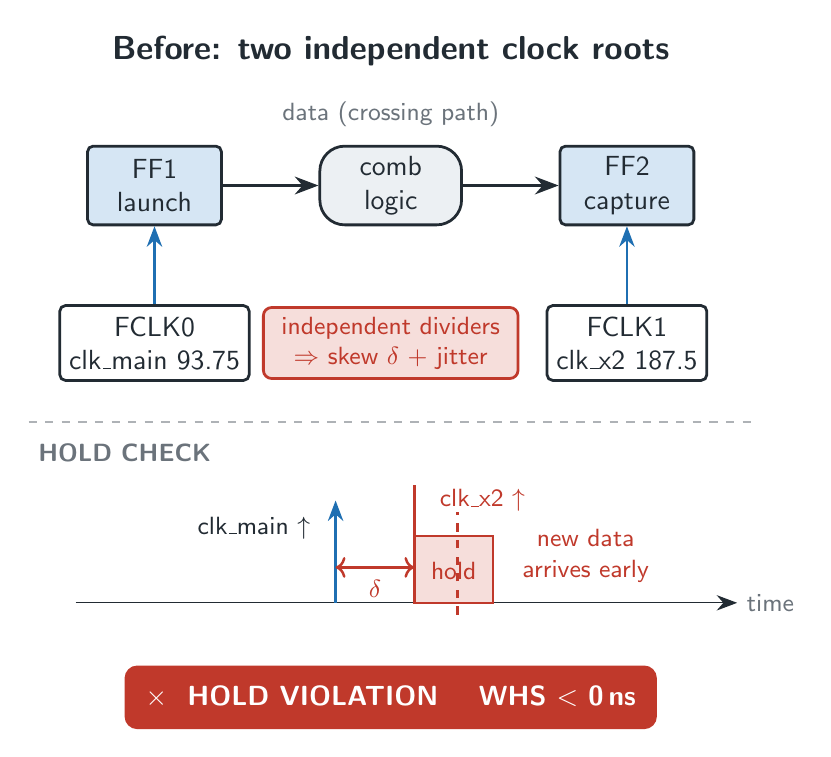
\begin{tikzpicture}[font=\sffamily]

  % ---- title ----
  \node[ttl] at (5,6.4) {Before: two independent clock roots};

  % ---- datapath ----
  \node[lab, text=mgrey] at (5,5.6) {data (crossing path)};
  \node[ff]  (ff1) at (2,4.7) {FF1\\launch};
  \node[cmb] (cmb) at (5,4.7) {comb\\logic};
  \node[ff]  (ff2) at (8,4.7) {FF2\\capture};
  \draw[data] (ff1.east) -- (cmb.west);
  \draw[data] (cmb.east) -- (ff2.west);

  % ---- two separate clock sources, fed straight up into the FFs ----
  \node[src] (f0) at (2,2.7) {FCLK0\\clk\_main 93.75};
  \node[src] (f1) at (8,2.7) {FCLK1\\clk\_x2 187.5};
  \draw[clk] (f0.north) -- (ff1.south);
  \draw[clk] (f1.north) -- (ff2.south);

  % ---- the problem ----
  \node[badnote] at (5,2.7) {independent dividers\\$\Rightarrow$ skew $\delta$ + jitter};

  % ---- divider ----
  \draw[divider] (0.4,1.7) -- (9.6,1.7);
  \node[sub, anchor=west] at (0.4,1.3) {HOLD CHECK};

  % ================= hold-check timeline =================
  \draw[-{Stealth[length=2.6mm]}, draw=dark] (1,-0.6) -- (9.4,-0.6)
        node[right, font=\sffamily\small, text=mgrey] {time};

  % launch (clk_main) and capture (clk_x2) edges -- offset by skew
  \draw[clk]  (4.3,-0.6) -- (4.3,0.7);
  \draw[memr, line width=1pt] (5.3,-0.6) -- (5.3,0.9);
  \node[lab,  anchor=east] at (4.1,0.35) {clk\_main $\uparrow$};
  \node[labr, anchor=west] at (5.5,0.7)  {clk\_x2 $\uparrow$};
  \draw[<->, memr, line width=0.9pt] (4.3,-0.15) -- (5.3,-0.15)
        node[midway, below=1pt, font=\sffamily\small, text=memr] {$\delta$};

  % hold window (red) + data that arrives too early (inside the window)
  \fill[lred] (5.3,-0.6) rectangle (6.3,0.25);
  \draw[memr, line width=0.9pt] (5.3,-0.6) rectangle (6.3,0.25);
  \node[labr] at (5.8,-0.2) {hold};
  \draw[memr, line width=1.3pt, dashed] (5.85,-0.75) -- (5.85,0.55);
  \node[labr, anchor=west] at (6.55,0.0) {new data\\arrives early};

  % ---- verdict ----
  \node[badchip] at (5,-1.8) {$\times$\ \ HOLD VIOLATION \quad WHS $<$ 0\,ns};

\end{tikzpicture}

% =====================================================================
% PAGE 2  --  AFTER : single MMCM root  ->  HOLD MET
% =====================================================================
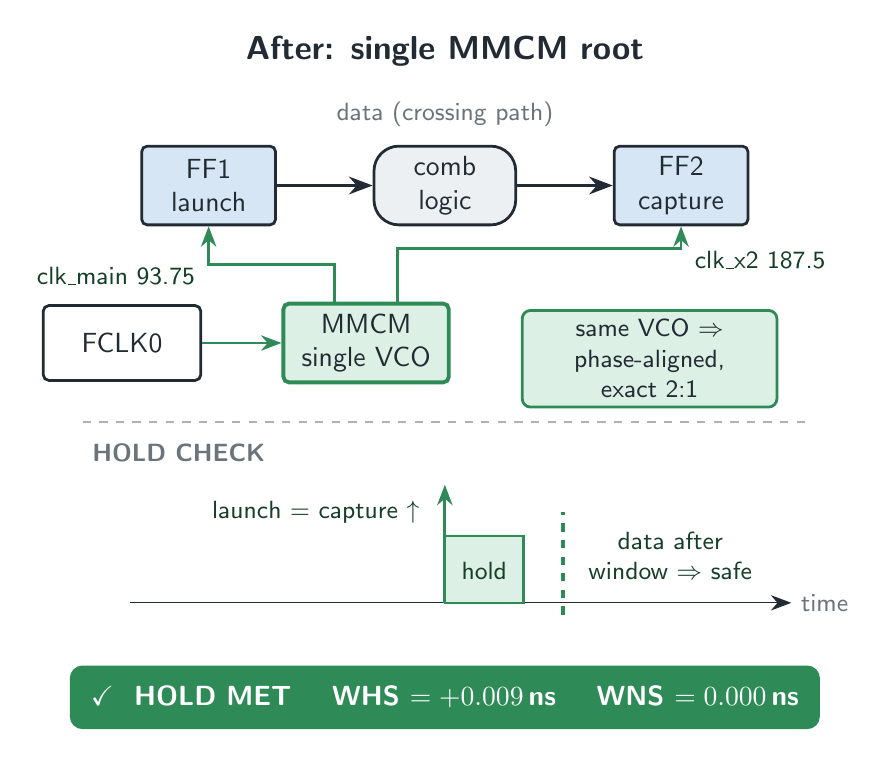
\begin{tikzpicture}[font=\sffamily]

  % ---- title ----
  \node[ttl] at (5,6.4) {After: single MMCM root};

  % ---- same datapath ----
  \node[lab, text=mgrey] at (5,5.6) {data (crossing path)};
  \node[ff]  (ff1) at (2,4.7) {FF1\\launch};
  \node[cmb] (cmb) at (5,4.7) {comb\\logic};
  \node[ff]  (ff2) at (8,4.7) {FF2\\capture};
  \draw[data] (ff1.east) -- (cmb.west);
  \draw[data] (cmb.east) -- (ff2.west);

  % ---- one source -> MMCM -> two phase-locked outputs (orthogonal routing) ----
  \node[src]  (f0)   at (0.9,2.7) {FCLK0};
  \node[mmcm] (mmcm) at (4.0,2.7) {MMCM\\single VCO};
  \draw[clkg] (f0.east) -- (mmcm.west);
  % left output  -> clk_main -> FF1   (up, left, up)
  \draw[clkg] (3.6,3.2) -- (3.6,3.7) -- (2,3.7) -- (ff1.south);
  % right output -> clk_x2  -> FF2   (up, right, up)
  \draw[clkg] (4.4,3.2) -- (4.4,3.9) -- (8,3.9) -- (ff2.south);
  \node[labg, anchor=east] at (1.95,3.55) {clk\_main 93.75};
  \node[labg, anchor=west] at (8.05,3.75) {clk\_x2 187.5};

  % ---- the fix ----
  \node[goodnote] at (7.6,2.5) {same VCO $\Rightarrow$\\phase-aligned, exact 2:1};

  % ---- divider ----
  \draw[divider] (0.4,1.7) -- (9.6,1.7);
  \node[sub, anchor=west] at (0.4,1.3) {HOLD CHECK};

  % ================= hold-check timeline =================
  \draw[-{Stealth[length=2.6mm]}, draw=dark] (1,-0.6) -- (9.4,-0.6)
        node[right, font=\sffamily\small, text=mgrey] {time};

  % launch and capture edges now coincident
  \draw[clkg] (5.0,-0.6) -- (5.0,0.9);
  \node[labg, anchor=east] at (4.8,0.55) {launch = capture $\uparrow$};

  % hold window (green) + data that arrives after the window -> safe
  \fill[lgrn] (5.0,-0.6) rectangle (6.0,0.25);
  \draw[grn, line width=0.9pt] (5.0,-0.6) rectangle (6.0,0.25);
  \node[labg] at (5.5,-0.2) {hold};
  \draw[grn, line width=1.3pt, dashed] (6.5,-0.75) -- (6.5,0.55);
  \node[labg, anchor=west] at (6.7,0.0) {data after\\window $\Rightarrow$ safe};

  % ---- verdict ----
  \node[goodchip] at (5,-1.8)
      {\checkmark\ \ HOLD MET \quad WHS $=+0.009$\,ns \quad WNS $=0.000$\,ns};

\end{tikzpicture}

\end{document}
